\documentclass[a4paper, 12pt]{article}
\usepackage{xeCJK}
\usepackage{hyperref}
\usepackage{indentfirst}
\usepackage{listings}
\usepackage{graphicx}
\usepackage{amsmath}
\usepackage{amsfonts}
\usepackage{amssymb}
\usepackage{multirow}
\usepackage{geometry}
\geometry{left=2cm, right=2cm, top=2.5cm, bottom=2.5cm}
\linespread{1.2}
\setlength{\parindent}{2em}
\title{基于支持向量机与卷积神经网络的\\汽油辛烷值定量分析\footnote{本项目托管于\url{https://github.com/sjx95/NIR-gasoline-RON-analysis}}}
\author{宋建勋\thanks{Email: \href{mailto:sjx95@outlook.com}{sjx95@outlook.com}} \\ \small(浙江大学, 浙江~杭州, 310027)}
\date{\small 2017 年 11 月 5 日}
\begin{document}
	\maketitle
	
	\begin{abstract}
		本文简要介绍了支持向量机与卷积神经网络的工作原理,然后对实验数据进行了必要的预处理,并使用支持向量回归和卷积神经网络两种方法构建了光谱与辛烷值之间的模型,并对两者的结果进行了评价与分析。
		其中支持向量机的回归误差复相关系数达到了 $R^2=0.9746$ ,而卷积神经网络则达到了 $R^2=0.9921$,均优于主成分回归等大部分统计学方法。
		作为两种通用的模型,这两者均较好的解决了近红外光谱的分析问题,达到了较为满意的精度。
	\end{abstract}
	
%	\tableofcontents
	
	\section{引言}
		汽油辛烷值是衡量汽油在气缸内抗爆震燃烧能力的一种指标,其值的高低意味着抗爆性的好坏。汽油在气缸中爆震燃烧时引起气缸温度剧升、汽油燃烧不完全、机器强烈震动,从而使输出功率下降,并容易造成机件受损。
		
		目前快速检测汽油辛烷值的方法主要有有红外光谱法、气相色谱法等。近红外光谱法由于成本低廉、速度快、无排放物等优点,逐渐成为车用汽油辛烷值测定的主流技术。然而由于近红外光谱的测量结果维数较多,各维度间具有一定程度的相关性,因此数据的分析处理则较为困难,基本的统计学方法如线性回归、主成分分析等效果一般。
		
		支持向量机 (Support Vector Machine, SVM) 是 Corinna Cortes 和 Vapnik 等于 1995 年首先提出的,它在解决小样本、非线性及高维模式识别中表现出许多特有的优势,并能够推广应用到函数拟合等其他机器学习问题中。支持向量机能够根据有限的样本信息在模型的复杂性和学习能力之间寻求最佳折中,以求获得较好的适应能力。
		LeNet 结构的卷积神经网络模型在 1986 年被提出,用于解决手写字体识别的问题。随后,各种结构的卷积神经网络被提出,用于解决各种图像分类问题。由近红外光谱的原理决定了近红外数据和图像数据在特征上具有一定的相似性,因此卷积神经网络也应当可以用于光谱分析。
		
	\section{工作环境}
		\noindent 本文使用的软件平台如下:
		
		\begin{itemize}
			\item openSUSE Tumbleweed + Linux Kernel 4.13.9
			\item Python 3.6 + pip
			\item libsvm
			\item Keras + TensorFlow
		\end{itemize}
	
		\subsection{openSUSE Tumbleweed + Linux Kernel 4.13.9}
			Linux 是一套开源的类 Unix 操作系统,它遵循 POSIX 标准,并具有对多用户、多任务、多线程和多CPU的支持。 
			openSUSE 则是基于 Linux 的发行版中的一套,其界面较为友好,比较易于使用。
		\subsection{Python}
			Python 是一种面向对象的解释型计算机程序设计语言,其源代码和解释器 CPython 遵循 GPL (GNU General Public License) 协议开源。
			Python 对科学计算具有良好的支持,拥有诸如 NumPy 、 SciPy 、 MatPlotLib 等诸多开源代码库。
			另外,它还能轻松的调用来自其他语言(比如C)所编写的库,即便于代码复用,还可以提高关键代码的运行速度。
		\subsection{libsvm}
			libsvm是台湾大学林智仁 (Lin Chih-Jen) 教授等开发设计的一个简单、易于使用和快速有效的SVM模式识别与回归的软件包,提供了包括C/Java/Python/MATLAB等大量接口,并基于 BSD 协议开源,其代码托管于\url{https://github.com/cjlin1/libsvm}。
			由于作者未通过PyPI提供包,需要参照手册自行编译并安装。
		\subsection{Keras + TensorFlow}
			TensorFlow 最初由 Google 大脑小组的研究员和工程师们开发出来,用于机器学习和深度神经网络方面的研究,但这个系统的通用性使其也可广泛用于其他计算领域。它灵活的架构让你可以在多种平台上展开计算,例如台式计算机中的一个或多个CPU(或GPU),服务器,移动设备等等。
			
			Keras 是一个高层神经网络 API , Keras 由纯 Python 编写而成并基于 Tensorflow 、 Theano 以及 CNTK 后端。Keras 为支持快速实验而生,能够把你的idea迅速转换为结果,具有高度模块化,极简,和可扩充特性,非常适合于简易和快速的原型设计。
			
	\section{数据预处理}
		光谱仪所采集的原始光谱图,除了受样品自身的基团组成与含量影响外,还会被样品颜色与杂质、检测器噪声所干扰。此外,光源强度、探头与样品的矩离、检测器灵敏度等因素也影响着光谱的强度。因此在对光谱进行建模前,需要通过适当的手段进行预处理,以便消除光谱数据中与样品基团组成无关的信息。
		
		本文使用的汽油 NIR 光谱数据如图\ref{fig:nir-data-raw}所示。
		
		\begin{figure}
			\centering
			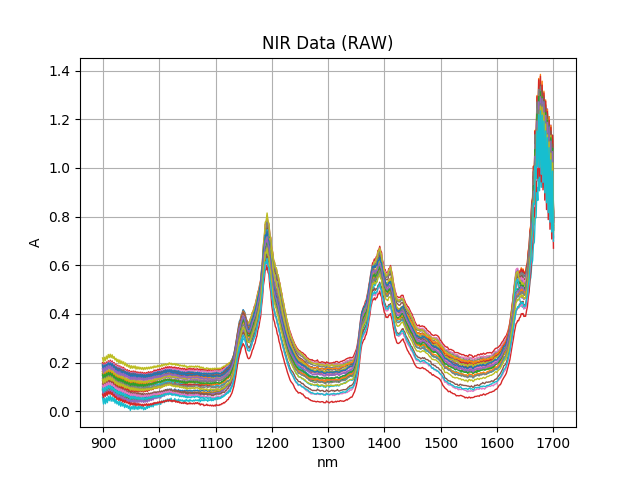
\includegraphics[width=0.8\linewidth]{../img/raw}
			\caption{原始光谱数据}
			\label{fig:nir-data-raw}
		\end{figure}
	
		\subsection{平滑}\label{section:filter}
			与图像处理或时域信号的预处理方式不同,光谱一般采用多项式卷积平滑进行预处理。
			多项式卷积平滑是通过对移动窗口内的数据进行多项式最小二乘拟合,以拟合值代替原始数据点,减少原始数据所含噪声对谱图的影响,达到平滑之目的。
			
			假设移动窗口的中心波长为 k ,半宽为 h ,再假定使用二次多项式进行拟合,则可以按公式 \eqref{equ:filter}来计算拟合参数。
			
			\begin{equation}\label{equ:filter}
				\beta_{LS}(k) = 
				\begin{bmatrix}
					a_0(k) \\ a_1(k) \\ a_2(k)
				\end{bmatrix}
				= \left( A(h)^TA(h) \right)^{-1}A(h)^TX(k) = 
				\begin{bmatrix}
					f_0(h) \\ f_1(h) \\ f_2(h)
				\end{bmatrix} 
				X(K)
			\end{equation}
			其中:
			\[
				A(h) =
				\begin{bmatrix}
					1 & -h & h^2 \\
					\vdots & \vdots & \vdots \\
					1 & 0 & 0 \\
					\vdots & \vdots & \vdots \\
					1 & h & h^2 \\
				\end{bmatrix} 
			\]
			
			在计算出拟合参数后,该点在平滑后的值则由公式\eqref{equ:filter2}得出。
			对图\ref{fig:nir-data-raw}中的数据进行平滑,取移动窗口半宽 $h = 5nm$ 得到的结果如图\ref{fig:filter}所示。
			可以看到,相比于图\ref{fig:nir-data-raw}中的原始数据,多项式卷积平滑有效的降低了噪声。
			
			\begin{equation}\label{equ:filter2}
				x_f(k) = a_0(k) = f_0(h)X(k)
			\end{equation}
			
			\begin{figure}
				\centering
				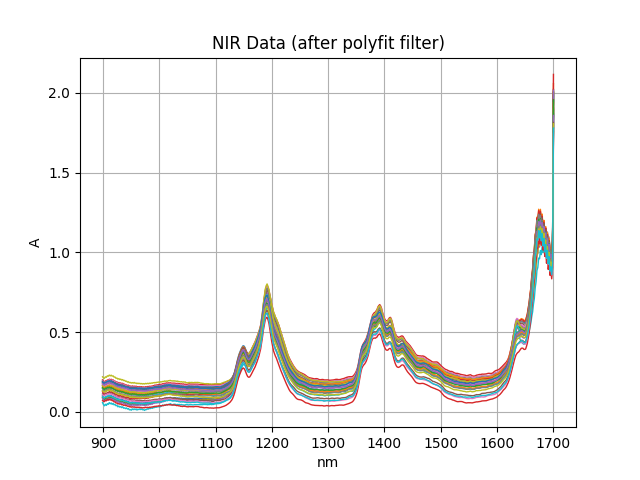
\includegraphics[width=0.8\linewidth]{../img/filter}
				\caption{光谱数据多项式卷积平滑结果}
				\label{fig:filter}
			\end{figure}
			
		\subsection{基线校正}
			由于光谱法一次测量的时间相对较长,若在这段时间内,各器件的特性可能会逐渐发生微小变化,这就会造成基线漂移。
			
			出于模型的健壮性考量,假定基线只发生了线性漂移,因此这里多次使用了一次多项式拟合进行迭代。对于每次拟合,可以认为原始数据落在拟合直线上方,且偏差超过拟合结果的均方根误差 (RMSE) 的点一定不属于基线,因此需要在下次拟合时忽略这些点;而其他的点则可能属于基线,应当参与下次拟合。随着迭代的进行,剔除的不属于基线的点越来越多,拟合结果也越来越靠近真实的基线。当拟合的均方根误差 (RMSE) 接近仪器的准确度时,继续迭代则会剔除掉原本属于基线的点,造成基线的偏离,因此应当停止迭代。
			
			基线校正的结果如图\ref{fig:baseline}所示,与图\ref{fig:nir-data-raw}所示的原始数据相比,各牌号汽油的光谱曲线均大致重合,较为符合实际情况。
			
			\begin{figure}
				\centering
				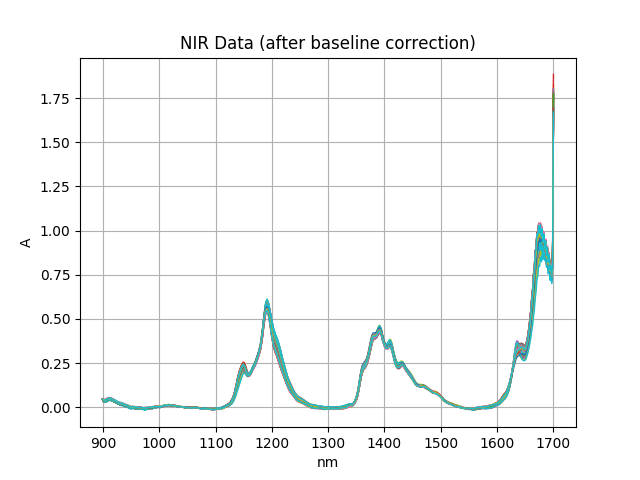
\includegraphics[width=0.8\linewidth]{../img/baseline}
				\caption{光谱数据基线校正结果}
				\label{fig:baseline}
			\end{figure}
			
		\subsection{微分}
			由于光谱数据的噪声较大,不太适合直接进行微分运算,因此需要先进行多项式平滑,然后再微分。多项式平滑的方法在第\ref{section:filter}节中已有叙述,只需在使用公式\ref{equ:filter2}计算输出值前,对拟合函数进行微分即可。
			
			因此首先使用公式\ref{equ:filter}计算每个中心波长的拟合参数,然后用公式\eqref{equ:diff}计算光谱当前波长的一阶微分值,或用公式\eqref{equ:diffdiff}计算光谱当前波长的二阶微分值。
			
			\begin{equation}\label{equ:diff}
				\frac{d\hat{x}(k+t)}{dt}\bigg|_{t=0}
				= a_1(k) =
				f_1(h)X(k)
			\end{equation}
			
			\begin{equation}\label{equ:diffdiff}
				\frac{d^2}{dt^2}\hat{x}(k+t)
				= 2a_2(k) =
				2f_2(h)X(k)
			\end{equation}
			
			光谱一阶微分后的结果如图\ref{fig:diff}所示,由于一阶微分获取的是变化量,因此除了滤波外,还消除了基线漂移的影响。
			
			\begin{figure}
				\centering
				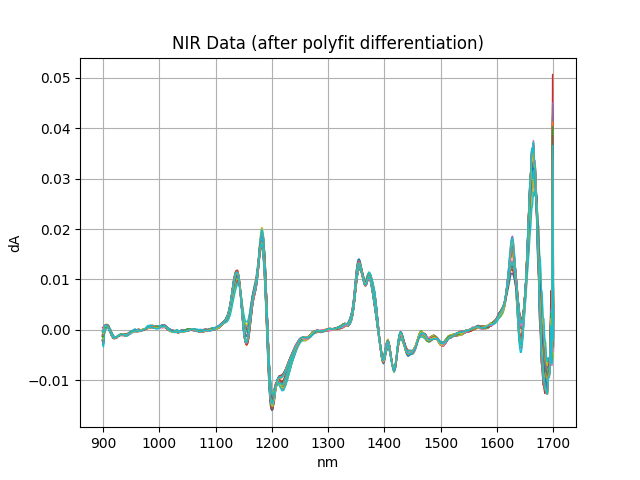
\includegraphics[width=0.8\linewidth]{../img/diff}
				\caption{光谱数据一阶微分结果}
				\label{fig:diff}
			\end{figure}
			
		\subsection{相关性分析}
			相关性分析用于考察光谱信息与待测参数的相关程度。若光谱各频率与待测参数的相关性均非常低,那么无论使用什么算法,通过分析光谱数据来获得待测参数都会非常困难。
			
			取每一个波长的数据,根据公式\eqref{equ:correlation}计算该波长上数据的相关性,其结果如图\ref{fig:correlation}所示。可以看到,在许多波长上,吸光度的一阶微分与待测参数的相关性显著,在 1220nm 附近甚至达到了 1 ,因此可以认为通过光谱来测量待测参数是可行的。
			
			\begin{equation}\label{equ:correlation}
				\rho_{XY} = \frac{Cov(X, Y)}{\sqrt{D(X)D(Y)}}
			\end{equation}
			\begin{figure}
				\centering
				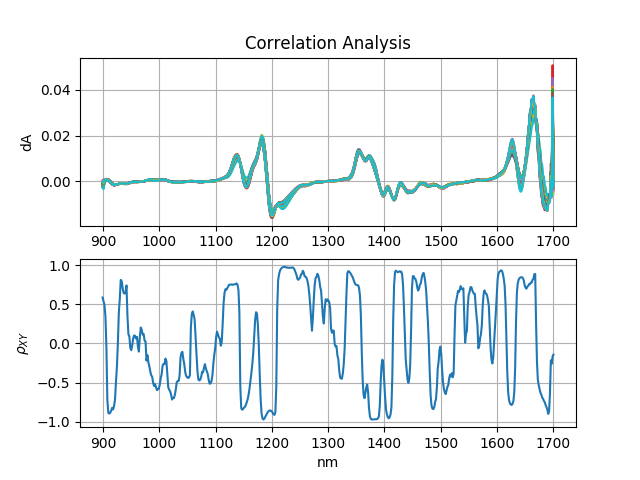
\includegraphics[width=0.8\linewidth]{../img/correlation}
				\caption{一阶微分的相关性分析}
				\label{fig:correlation}
			\end{figure}
			
	\section{支持向量机}
		\subsection{相关理论}
			支持向量机是用来解决二分类问题的一种模型,其中线性支持向量分类机用于处理线性可分问题,或在一定的允许误差下处理线性近似可分问题。线性支持向量分类机的核心思想在于寻找间隔最大的两张平行的超平面,使得两类样本各自分居在两张超平面的两侧,此时选取与这两张超平面距离相等且平行的一张超平面,即可将样本妥善的划分开来。而支持向量则指的是数据集中支撑起两张超平面的那些样本点,对于一个确定的数据集,其超平面的划分则只与支持向量有关,与非支持向量无关。
			
			为了处理线性近似可分的问题,可以适当放宽线性支持向量机构造超平面时的约束条件,即允许某些样本点越过超平面。假定每个样本点越过相应超平面的距离为 $\xi_i \geqslant 0$ ,那么总存在一个足够大的 $\xi_i$ ,使得某一满足约束条件的超平面划分存在。但是,显然应该避免 $\xi_i$取得太大,因此需要在目标函数中引入 $\sum\left(\xi_i\right)$ 作为惩罚。这样,线性支持向量机就可以被推广到解决近似线性可分的问题上。
			
			然而,对于有些分类问题明显不宜采用线性划分。
			如图\ref{fig:unlinear-dataset}所示落在 $R^2$ 空间上的数据集,理想的划分曲线应当为一个圆,若使用线性支持向量分类机,误差则会变得不可接受。
			由此引出了非线性支持向量分类机,其核心思想是寻找一个核函数,将线性不可分的数据集从原始空间映射到高维空间,使其变得线性可分。
			这样就可以继续使用线性支持向量分类机的方法,对数据集进行分类了。
			
			\begin{figure}[h]
				\centering
				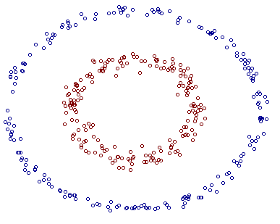
\includegraphics[width=0.5\linewidth]{img/线性不可分数据集}
				\caption{线性不可分数据集}
				\label{fig:unlinear-dataset}
			\end{figure}
			
			更进一步地,如果在映射的过程中,人为的在被映射到的高维空间中增加带测参数的维度,那么可以将支持向量分类机转换为支持向量回归机。原本的优化目标,即寻找最大间隔超平面,也就转变成了在新的高维空间中寻找一个超平面,使其距离各样本点的距离最小。这样,支持向量机除了可以解决分类问题,也就可以解决回归问题了。
			
		\subsection{实现方法}
			这里选用支持向量机的libsvm实现的Python接口。该接口主要提供了以下几个函数:
			\begin{itemize}
				\item svm\_train: 用于训练模型,其中参数由字符串的形式传入;
				\item svm\_predict: 用于预测数据,如果给出真值还可以评估模型效果;
				\item svm\_save\_model: 用于保存模型;
				\item svm\_load\_model: 用于加载模型。
			\end{itemize}
			其中, svm\_train 能够调整的主要参数有:
			\begin{itemize}\setlength{\itemsep}{0pt}
				\item -s svm\_type : 设置 SVM 类型 (default 0)
				\subitem 0 -- C-SVC		(多分类)
				\subitem 1 -- nu-SVC	(多分类)
				\subitem 2 -- 一分类 SVM
				\subitem 3 -- epsilon-SVR	(回归)
				\subitem 4 -- nu-SVR		(回归)
				\item -t kernel\_type : 设置核函数类型 (default 2)
				\subitem 0 -- 线性: $u'*v$
				\subitem 1 -- 多项式: $(\gamma * u' * v + coef0)^{degree}$
				\subitem 2 -- 径向基函数: $e^{-\gamma * \left|u-v\right|^2}$
				\subitem 3 -- sigmoid 函数: $\tanh(\gamma * u' * v+coef0)$
				\item -c cost : 设置 C-SVC、 epsilon-SVR 和 nu-SVR 的惩罚系数 (default 1)
			\end{itemize}

			显然,这里应选择 epsilon-SVR ,而核函数类型和惩罚系数还需要进行一些尝试才能选出一个较好的值。
			
		\subsection{训练结果与分析}
			由于支持向量机需要在进行训练和处理前对数据进行标准化,因此使用公式\eqref{equ:standard}对各维度进行标准化。然后再按照 libsvm 的格式要求,将输入数据由二维数组转换为字典列表的格式。为了防止模型过拟合,还需要将30条数据按 $2:1$ 划分为训练集和测试集,训练集用来训练模型,测试集用来检测训练效果。
			
			\begin{equation}\label{equ:standard}
				z = \frac{x - \mu}{\sigma}
			\end{equation}
			
			随后需要确定一个合适的核函数,这里分别尝试了四种核函数,使用默认参数进行训练,训练结果如图\ref{fig:svm_result_t}所示。
			
			由于Sigmoid核函数的效果最好,这里选择 Sigmoid 核函数并进一步调整惩罚系数。不同惩罚系数下的训练结果如图\ref{fig:svm_result_c}所示。当惩罚系数 $c = 1.6$时,模型的预测效果最好,其回归标准误差为0.4835,回归误差复相关系数为0.9746,与主成分回归效果相当。
			
			各模型的评价指标汇总如表\ref{table:svr_result}所示。考虑到监督学习模型中,模型的精确度一定程度上依赖于训练数据量,而这里能拿到的近红外光谱数据只有30条,如果能够拿到更多的数据,模型的准确度理应还存在一定的提升空间。
			
			\begin{figure}
				\centering
				\begin{minipage}{0.85\linewidth}
					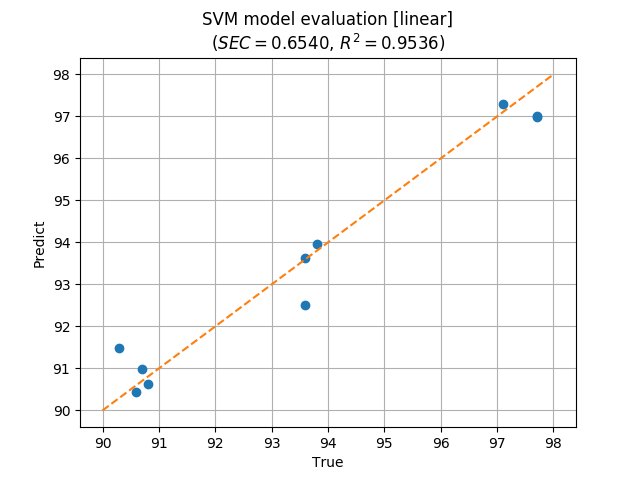
\includegraphics[width=0.5\linewidth]{../img/svm_result_t0}
					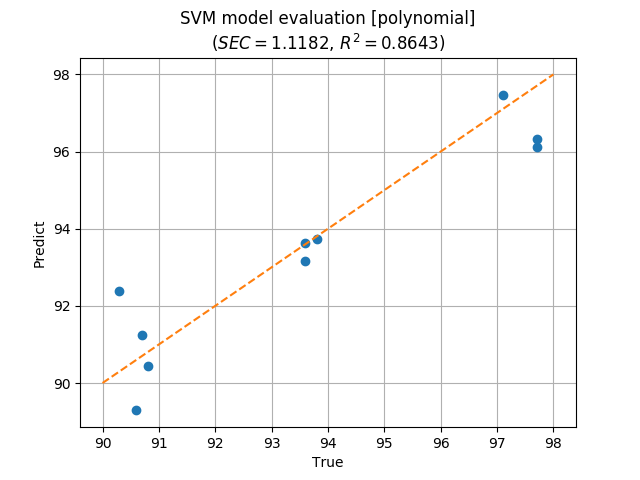
\includegraphics[width=0.5\linewidth]{../img/svm_result_t1}
					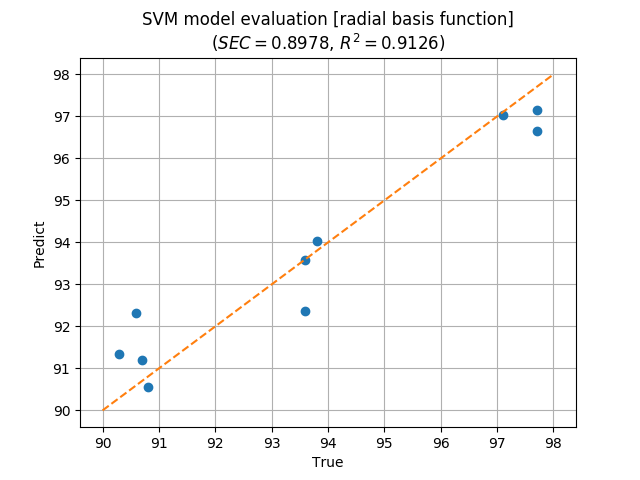
\includegraphics[width=0.5\linewidth]{../img/svm_result_t2}
					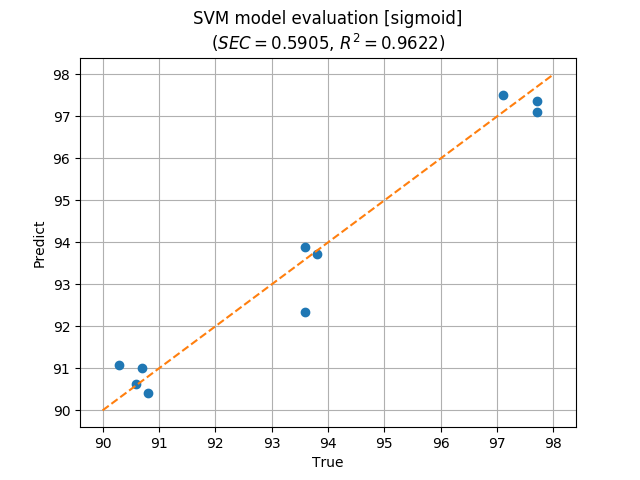
\includegraphics[width=0.5\linewidth]{../img/svm_result_t3}
				\end{minipage}
				\caption{各类核函数训练结果}
				\label{fig:svm_result_t}
			\end{figure}
			\begin{figure}
				\centering
				\begin{minipage}{0.85\linewidth}
					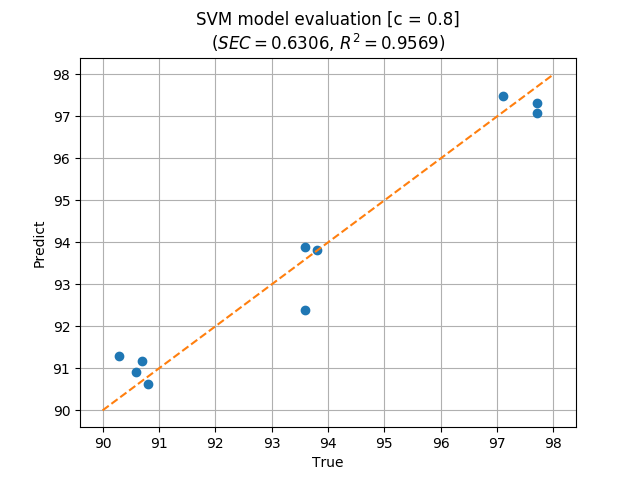
\includegraphics[width=0.5\linewidth]{../img/svm_result_t3_c0_8}
					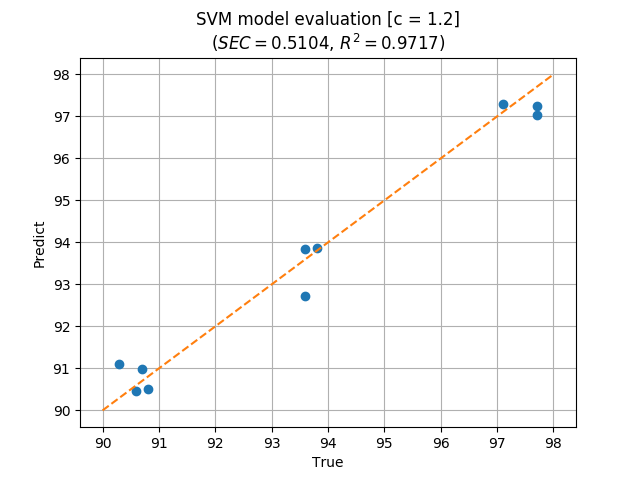
\includegraphics[width=0.5\linewidth]{../img/svm_result_t3_c1_2}
					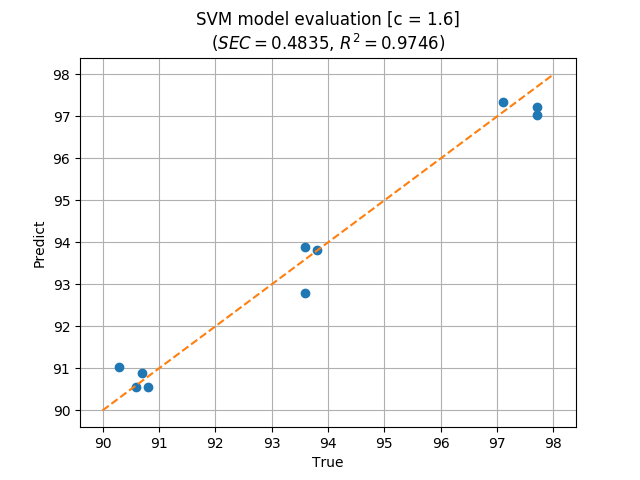
\includegraphics[width=0.5\linewidth]{../img/svm_result_t3_c1_6}
					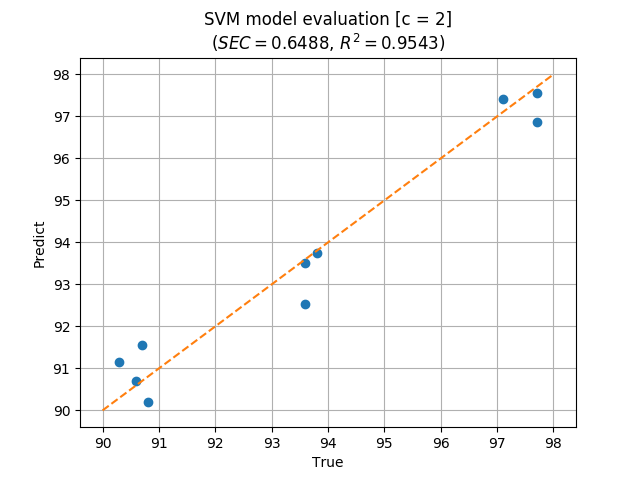
\includegraphics[width=0.5\linewidth]{../img/svm_result_t3_c2}
				\end{minipage}
				\caption{Sigmoid核函数在各惩罚系数下的训练结果}
				\label{fig:svm_result_c}
			\end{figure}
			
			\begin{table}[h]
				\caption{SVM训练结果汇总}
				\label{table:svr_result}
				\centering
				\begin{tabular}{r|c|c|c|c|c|c|c|c}
					\hline
					核函数&线性&多项式&径向基&\multicolumn{5}{c}{Sigmoid} \\
					\hline
					惩罚系数&\multicolumn{4}{c|}{$c = 1$}&0.8&1.2&1.6&2\\
					\hline
					SEC&0.6540&1.1182&0.8978&0.5905&0.6306&0.5104&0.4835&0.6488\\
					$R^2$&0.9536&0.8643&0.9126&0.9622&0.9569&0.9717&0.9746&0.9543\\
					\hline
				\end{tabular}
			\end{table}

	\section{卷积神经网络}
		卷积神经网络 (Convolutional Neural Network, CNN) 是一种前馈神经网络,常被用在处理图像数据的神经网络中。相比于 BP 神经网络,针对图像数据相邻像素点间具有关联性这一特征, CNN 增加了卷积层和池化层,用于提取相邻像素点间的关联并降低网络的总特征数。
		在光谱数据处理中,由于样品在相邻波长的响应也具有关联性,因此卷积神经网络也应当适用于光谱分析。
		
		\subsection{网络结构}
			理论上,只要特征数目足够多,神经网络在大量数据下都会具有较好的表现。然而在实际情况下,结构不佳的神经网络,很可能会由于训练数据不足导致效果不佳,也有可能会落入局部最优解,甚至有可能无法收敛。因此,安排一个合理的网络结构是很重要的。
			
			这里参考 LeNet 的网络结构,首先进行了4次卷积+池化操作,然后经过全连接层到达输出层。其中,激活函数选用了 ReLu ,损失函数选用了 MSE ,优化器选用了 Adam 。为了防止模型过拟合,当精度经过连续数轮训练没有改善时,还要及时提前停止训练。整个网络的结构如下:
			
			\noindent \begin{minipage}{\linewidth}
				\lstinputlisting[]{../cnn-model.txt}
			\end{minipage}
				

		\subsection{训练结果与分析}
			为了提高拟合速度,在开始训练前,需要使用公式\eqref{equ:standard}对每条光谱数据进行标准化。随后按照 TensorFlow 的格式,将输入数据组织为数组的形式。
			为了防止模型过拟合,还需要将 30 条数据按 $2:1$ 划分为训练集和测试集,训练集用来训练模型,测试集用来检测训练效果。
			
			相比于 SVM , CNN 的结构更复杂,参数也更多,因此训练需要的迭代次数也更多,训练时间也更长。另外, CNN 的训练方法也意味着训练结果具有一定程度的随机性,可能需要多尝试几次才能拿到比较好的模型。
			
			最终模型的交叉检验结果如图\ref{fig:cnnresult}所示,其回归标准误差为0.2694,回归误差复相关系数为0.9921,优于主成分回归和支持向量回归,但与主元数较多时的偏最小二乘回归还有一定的差距。
			
			\begin{figure}
				\centering
				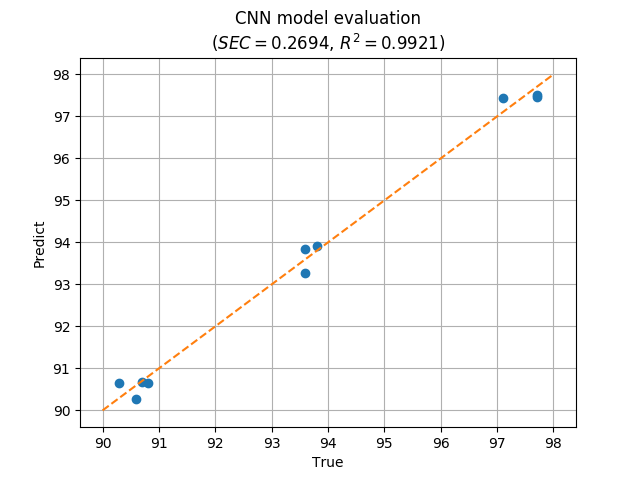
\includegraphics[width=\linewidth]{../img/cnn_result}
				\caption{CNN训练结果}
				\label{fig:cnnresult}
			\end{figure}
			
			一般来说,神经网络需要比支持向量回归更多的训练数据,然而这里 CNN 的表现却比支持向量回归更好。这可能是由于 CNN 的卷积层相比于全连接层,能够更加有效的提取光谱的特征,大幅降低了神经网络中的参数量,使得少量数据也能够有效提取到特征。另外从原理上来看,相比于 SVM ,CNN 的塑性也更好。
			
	\section{总结}
		本文首先对获取的实验数据进行了必要的预处理,然后尝试使用了支持向量回归和卷积神经网络两种方法来构建光谱与辛烷值之间的模型,其模型的预测精度汇总于表\ref{table:model-compare}。同时还对两者的结果进行了一定的对比分析。支持向量机与卷积神经网络作为两种通用的模型,均较好的解决近红外光谱的分析问题,不仅达到了较为满意的精度,在继续加大数据量的同时,还有着进一步提升的空间。
		
		\begin{table}
			\caption{各模型精度对比}
			\label{table:model-compare}
			\centering
			\small
			\begin{tabular}{r|c|c|c|c|c|c|c|c||c|c}
				\hline
				\multicolumn{9}{c||}{SVR} & \multicolumn{1}{c|}{\multirow{3}{*}{CNN}} \\
				\cline{1-9}
				核函数&线性&多项式&径向基&\multicolumn{5}{c||}{Sigmoid}& \\
				\cline{1-9}
				惩罚系数&\multicolumn{4}{c|}{$c = 1$}&0.8&1.2&1.6&2& \\
				\hline
				SEC&0.6540&1.1182&0.8978&0.5905&0.6306&0.5104&0.4835&0.6488&0.2694&SEC\\
				$R^2$&0.9536&0.8643&0.9126&0.9622&0.9569&0.9717&0.9746&0.9543&0.9921&$R^2$\\
				\hline
			\end{tabular}
		\end{table}
		
		然而需要注意的是,作为通用的代价,训练这两种模型均需要大量的数据。由于本文仅有某台仪器某品牌油品测出的30组数据作为样本数据,尽管划分训练集和测试集后,在测试集上的预测效果不错,但拿到另一台仪器或者测试另一品牌油品时是否可靠还有待验证。而且神经网络模型相较于统计模型,其内部联系非常复杂,误差的追溯甚至难以进行,也难以给出有效的机理分析。
		不过也正是因为这种通用性,在应用环境发生变化时,无需重新进行统计分析,只需要在原来模型的基础上,追加新的训练数据即可重新达到原有精度。
		
	\small
	\renewcommand{\refname}{参考资料}
	\begin{thebibliography}{9}
		\bibitem{} 在线分析技术及仪器 - 课程讲义
		\bibitem{} 邓乃扬, 田英杰. 支持向量机:理论、算法与拓展[M]. 科学出版社, 2009.
		\bibitem{} July, pluskid. 支持向量机通俗导论(理解SVM的三层境界)[EB/OL]. [2017-11-05]. \url{http://blog.csdn.net/macyang/article/details/38782399/}.
		\bibitem{} \href{https://github.com/fchollet}{fchollet}. Keras Documentation[EB/OL]. [2017-11-05]. \url{https://keras.io/}.
	\end{thebibliography}
\end{document}